\documentclass{article}




% ------ PACKAGES ------


\usepackage{subfigure}

\usepackage{fullpage}
\usepackage{parskip}
\usepackage{titlesec}
\usepackage{xcolor}
\usepackage[colorlinks = true,
            linkcolor = blue,
            urlcolor  = blue,
            citecolor = blue,
            anchorcolor = blue]{hyperref}
\usepackage[natbibapa]{apacite}
\usepackage{eso-pic}

\renewenvironment{abstract}
  {{\bfseries\noindent{\abstractname}\par\nobreak}\footnotesize}
  {\bigskip}

\titlespacing{\section}{0pt}{*3}{*1}
\titlespacing{\subsection}{0pt}{*2}{*0.5}
\titlespacing{\subsubsection}{0pt}{*1.5}{0pt}

\usepackage{authblk}

\usepackage{graphicx}
\usepackage[space]{grffile}
\usepackage{latexsym}
\usepackage{textcomp}
\usepackage{longtable}
\usepackage{tabulary}
\usepackage{booktabs,array,multirow}
\usepackage{amsfonts,amsmath,amssymb}
\providecommand\citet{\cite}
\providecommand\citep{\cite}
\providecommand\citealt{\cite}
% You can conditionalize code for latexml or normal latex using this.
\newif\iflatexml\latexmlfalse
\providecommand{\tightlist}{\setlength{\itemsep}{0pt}\setlength{\parskip}{0pt}}%

\AtBeginDocument{\DeclareGraphicsExtensions{.pdf,.PDF,.eps,.EPS,.png,.PNG,.tif,.TIF,.jpg,.JPG,.jpeg,.JPEG}}

\usepackage[utf8]{inputenc}
\usepackage[english]{babel}



\begin{document}

\title{Cost-effective model building in multivariate calibration}


\author[ ]{Valeria Fonseca Diaz, Bart De Ketelaere, Ben Aernouts, Wouter Saeys}

\affil[ ]{}
\vspace{-1em}


\date{}

\begingroup
\let\center\flushleft
\let\endcenter\endflushleft
\maketitle
\endgroup

\selectlanguage{english}
\begin{abstract}
{
Multivariate calibration models conceived as virtual sensors that are used to measure chemical compositions in products are built based on spectral data of samples and their corresponding reference chemical values. The cost of these reference analyses is a major of feature of interest to be minimized in industrial applications for the sake of more efficient analytical processes. The present work aims at characterizing the problem of sample selection based on spectral measurements to build calibration models. We mainly focused on evaluating optimal sample sizes, evaluation of different selection methods and we give recommendations on how to assess the suitability of a set of samples to build bilinear calibration models.
}\\%
\end{abstract}%



\section*{Introduction}\label{introduction}

Multivariate calibration models have been the primary analytical tool to indirectly measure the chemical composition of products making processes such as those of quality control more cost-efficient. Many are still the challenges that are present when building and maintaining these models. In the present work, we aim to make an exhaustive evaluation of the problem of unsupervised sample selection to build successful calibration models. 

Among the different applications where multivariate calibration models take place, the sample collection problem van be regarded as one of designing the samples and as another one of collecting the samples. The first one is the type of problem concerning pharmaceutical applications or in general chemical preparations. The second one is the type of problem that takes place in the agrofood industry (AFI) such as fruits quality inspections, determination of harvesting periods, soil quality, among others. 

Within the second type of applications, the problem of unsupervised sample selection consists in determining what the best methodology is to select the samples that would be worthy for reference analysis only based on spectral measurements. As it is widely known, spectral measurements are easy and cheap to collect, therefore a vast quantity of units can be submitted to these measurements with low effort. On the contrary, collecting the reference analyses is a task that requires a lot of effort, high costs and possibly high waste. 

To set the scope of the present analysis, this work is developed under the sphere of bilinear multivariate calibration models for regression, that is, partial least squares regression (PLSR). This means that conclusions on the optimality of a set of samples to build a model are drawn in light of the particular model type and architecture. Although results are not presented here for non-linear models in regression or even for the problem of classification, the same ideas that will be presented can be analysed in those particular cases. 

PLSR is the most common method or algorithm used to build a bilinear regression model for high-dimensional spectral matrices to be connected to reference analyses. Although other algorithms for the linear model can be used or even consider the problem of a non-linear model, the linear relationship solved by PLSR has proven to be optimal throughout the last decades in modeling the required relationship. 

We present here a general and a specific framework of PLSR in order to set a context of analysis to solve the problem of the best strategy for unsupervised sample selection. In the coming sections, we present the frameworks involved together with the research questions that they bring. Afterwards, the experimental work and results are presented along with the discussion and analysis on the aspects that lead to a more successful set of samples to build calibration models.


\section*{Frameworks to understand PLSR}

\subsection*{The general framework}

We aim to put PLSR in the general framework of statistical learning theory. As such, we assume that the response variable is a function consisting in a linear combination and an error variable. With that model architecture, the aim is to minimize a square error. More concretely, let $y \in \mathbb{R}$ be the random variable representing the reference chemical variable of interest and   $\mathbf{x} \in \mathbb{R}^{p}$ the predictor vector of spectral measurements. We assume the relationship $ y = f(\mathbf{x}, \boldsymbol{\beta}) + \epsilon$.  The general regression problem with square error can be established as:

\begin{equation}
    \min E \left[ (y-f(\mathbf{x}, \boldsymbol{\beta}))^2\right]; \quad f(\mathbf{x}, \boldsymbol{\beta}) = \sum_{k=1}^{\infty} \beta_k \phi_{k}(\mathbf{x})
    \label{eq_general_regression_problem}
\end{equation}

where $\{\phi_{i}(\mathbf{x})\}$ constitute a basis of $L_2$ which can be ordered by some criterion. In terms of the statistical learning theory by Vapnik, $E \left[ (y-f(\mathbf{x}, \boldsymbol{\beta}))^2\right]$ is called the \emph{expected risk} which is in practice replaced by the so-called \emph{empirical risk} in the presence of a set of $n$ observations to estimate function $f$. In this case, the empirical risk is what has been known for centuries as the sum of square errors. Now, to ensure a small \emph{expected risk}, the \emph{empirical risk} can be minimized only over a limited number of basis functions $\{\phi_{k}(\mathbf{x})\}_{k=1}^d$. Therefore, we are left with a regression problem of the form:

\begin{equation}
    \min \frac{1}{n} \sum_{i=1}^n (y_i-f_d(\mathbf{x}_i, \boldsymbol{\beta}))^2; \quad f_d(\mathbf{x}, \boldsymbol{\beta}) = \sum_{k=1}^{d} \beta_k \phi_{k}(\mathbf{x})
    \label{eq_square_loss_empirical_regression_problem}
\end{equation}

It is therefore in this regard, that the problem as stated in eq. (\ref{eq_square_loss_empirical_regression_problem}) corresponds to the problem that is solved with the PLSR algorithm, where the basis $\{\phi_{k}(\mathbf{x})\}$ is constructed based on finding the eigenvectors of the covariance between $y$ and $\mathbf{x}$ and are ordered by the amount of covariance. The key element in this framework is the fact that the number of chosen basis functions $d$ represents what Vapnik's theory calls the $VC$ dimension, which is a value that measures the capacity control of a learning machine. The importance of a capacity control value as $d$ for PLSR comes as the reference for determining a suitable sample size when aiming to build a regression machine or as known in the context of chemometrics, a multivariate calibration model. 

In Vapnik's work, it has been stated that we can talk about small sample size or a large sample size depending on the ratio between the sample size and the $VC$ dimension. Although there is no absolute threshold, it is stated that a large sample size starts when the ratio $n/d>20$.

% mention here the work found in the group of Tom Fearn, australia

\subsection*{The specific framework}

In the jargon of multivariate calibration, the basis of $L_2$ is what is known as the set of latent variables. Based on a set of $n$ observations stored in the matrices $\mathbf{X}_{n\times p}$ and $Y_{n\times 1}$, the underlying idea of the PLS algorithm is to build latent variables $\{\phi_{k}(\mathbf{x})\}$ such that $\phi_k(\mathbf{x}) = \mathbf{Xv}_{k}$, where $\mathbf{v}_k$ results from maximizing the covariance between $X$ and $Y$ at the $k$-th deflation step. 

For a given value of $d$, the set of resulting latent variables constitute a set of orthonormal variables $\{\phi_{k}(\mathbf{x})\}_{i=1}^d$. However, the set of loading vectors $\{\mathbf{v}_k\}$ is regarded as $\mathbf{S}$-orthogonal, i.e. $\mathbf{v}_k'\mathbf{S}\mathbf{v}_j = 0 \quad (j<k)$, where $\mathbf{S}$ is the covariance matrix of $\mathbf{X}$. The current depiction of the PLS algorithm clarifies that the estimation of the regression model depends highly on the covariance matrix $\mathbf{S}$ and therefore, when there is availability of a number of spectral measurements $N$, we can think of selecting a smaller amount of samples $n$ for reference analysis and expect to have a similar performance as long as there is equivalence of the matrices $\mathbf{S}$ from the larger sample to the smaller sample. 


\section*{Research questions}

When depicting the understanding of PLSR models from a general framework and a specific framework, we see that there are clear elements to take into account at the moment of selecting samples from a large set of available spectral measurements to build calibration models. On the one hand, the $VC$ dimension comes as a reference value for the sample size. On the other hand, if $N$ spectral measurements are available, we may be able to determine the quality of a set a subset of these samples of size $n<N$ based on the equivalence of the covariance matrices $\mathbf{S}$ for $N$ and $n$ samples concluding that the resulting PLSR model in the presence of $N$ analysis is not importantly different from the resulting model based on selected $n$ samples. With this in mind, our research questions are:

\begin{itemize}
    \item Can we find specific thresholds for the optimal sample size in particular for calibration models in chemometrics based on the ratio $n/d$?
    \item What are the most suitable selection methods in the state of the art for the sake of satisfactory PLSR models?
    \item How can we evaluate the equivalence between the matrices $\mathbf{S}$ of different sample sizes when using the sota methods for selection?
\end{itemize}

\section*{Experimental}\label{experimental}

\subsection*{Case studies}\label{data}

We selected two AFI real case studies to demonstrate the aspects previously discussed about unsupervised sample selection. The first one corresponds to the inspection of milk composition where data of 2 periods of time was available both for spectral signals and reference analysis. During the first period 316 samples were collected followed by 79 new samples collected in the second period. The time frame between the periods was one week. The spectral measurements correspond to transmittance mode gathered in the range 900 nm - 1700 nm with a resolution of 3 nm. In this case the chemical variable of interest was lactose. 
The second case corresponds to pig manure samples were 2 sets were available for the inspection of the manure composition. One set of 420 samples was measured under the same conditions for calibration and another set of 164 samples was measured for validation. The chemical constituent chosen for inspection through calibration was Dry Matter. The spectral measurements correspond to reflectance model in the range 426 nm - 1686 nm with a resolution of 9 nm.
For the purpose of analyzing the sample selection problem, we refer to the first sets in both cases as selection set, the samples chosen by the different methods constitute the calibration set and the samples on the second sets represent the test set. 

\textbf{Preprocessing:} For the purpose of studying unsupervised sample selection for satisfactory calibration models, only mean centering preprocessing was used in all cases. Intuitively and after a few experiments, it was seen that assuming certain preprocessing filters for the spectral measurements prior to any knowledge of the $y$ values might be harmful for the resulting model.

\subsection*{Methodology}\label{methodology}

\subsubsection*{Exhaustive evaluation for unsupervised sample selection}

We set up an exhaustive evaluation consisting in combining three main factors involved into the problem of interest: Method, input dimensionality and sample size. We aimed to evaluate the real impact of each of this factors by selecting subsets of samples for each possibility resulting from combining the different options of these factors.  

\textbf{Selection methods}

There are multiple methods in the state of the art for sample selection based on the available matrix $\mathbf{X}$. After revising the literature on chemometrics and calibration models, the methods selected for the present work were: Kennard Stone (KS), Duplex (D), Puchwein (P), complete linkage hierarchical clustering (CL) and D-optimal designs based on the optfederov algorithm (D-OPT). In addition, we included random selection (RS). 

\textbf{Input dimensionality}

The available spectral measurements stored in matrix $\mathbf{X}_{N\times p}$ correspond to an input dimensionality of $p$. However, due to the rank deficit of $\mathbf{X}$, it is also possible to reduce the input dimensionality for sample selection via principal component analysis (PCA) scores, therefore defining an input matrix $\mathbf{T}_{N\times a}$ of $a$ PC scores, which sets a range for the input dimensionality $a$. The value of $a$ should not be confused with the $VC$ dimension for the PLSR model $d$. Based on the evaluation of the current cases and results seen in the literature of chemometrics, the maximum number for $a$ was set to 25.

\textbf{Sample size}

The minimum sample size was set to 30 samples. The sample size range was considered in steps of 10 from 30 to the maximum number of samples available in the selection set for each case study. 

\textbf{Constraints}

For the distance-based selection methods (KS,D,P,CL), a mahalanobis distance was used when the input matrix was set to $\mathbf{T}$ and an euclidean distance measure was used for the input matrix $\mathbf{X}$. This is decided because the inverse of the covariance matrix $\mathbf{S}$ to be used in the mahalanobis distance becomes too unstable due to the rank deficiency. For the same reason, the selection based on OPT can be made only with input matrix $\mathbf{T}$. 

\begin{table*}[t]
\centering
\begin{tabular}{|c|c|c|} 
\hline
Selection method	& Input dimensionality	& Sample size	\\
\hline

KS & 1 PC   & 30  \\
D &  . & 40\\
P &  . & . \\
CL & . & . \\
D-OPT & 25 PC's & .\\
RS & $p$ & $N$\\
\hline


\end{tabular}
\caption{Sample selection settings}
\label{tab_samplesel_settings_exhaustive_search}
\end{table*}

\subsubsection*{Analysis of covariance matrix $\mathbf{S}$}

We evaluated the equivalence or congruence between the covariance matrix based on the full available sample of size $N$ ($\mathbf{S}_N$) and a covariance matrix based on a subset of size $n$ ($\mathbf{S}_n$) through the correspondence of their eigenvectors and the eigenvalues. The spectral value decomposition of $\mathbf{S}_N = \mathbf{V_N \Delta_N V'_N}$ and $\mathbf{S}_n = \mathbf{V_n \Delta_n V'_n}$ was calculated. The eigenvalues were compared by calculating the ratio  $\Delta_n/\Delta_N$ and the eigenvectors were compared by computing the absolute value of the determinant for the matrix $V'_nV_N$ setting a value for the rank. 

\subsubsection*{Multivariate calibration models}

The PLSR models were trained using the SIMPLS algorithm. For each selection setting as explained in table \ref{tab_samplesel_settings_exhaustive_search}, a PLSR model was calibrated with the selected samples and applied on the separated test set for each case study. The performance of the model corresponded to the root mean squared error (RMSE) on the test set in a range from 1 to 30 latent variables. 

\subsection*{Computational tools}

The complete analysis was programmed and run in Python 3.7. The selection methods, excluding D-OPT, were programmed in house as well as the SIMPLS algorithm. The D-OPT method was used in a connection from R to Python, using the function \texttt{optfederov} from the R-package \emph{AlgDesign}. The exhaustive sample selection and subsequent PLSR calibrations was embedded into a loop which was highly optimized using \texttt{numba} for Python. It was possible to fit more than 5000 PLSR models including crossvalidation results in 10 minutes in an 64-bit Inter Core i7 vPro 8th generation with 16 GB of RAM. 


\section*{Results}\label{results}

% descriptive statistics tables

\subsection*{General framework}\label{results:genframework}

\begin{figure}[b]
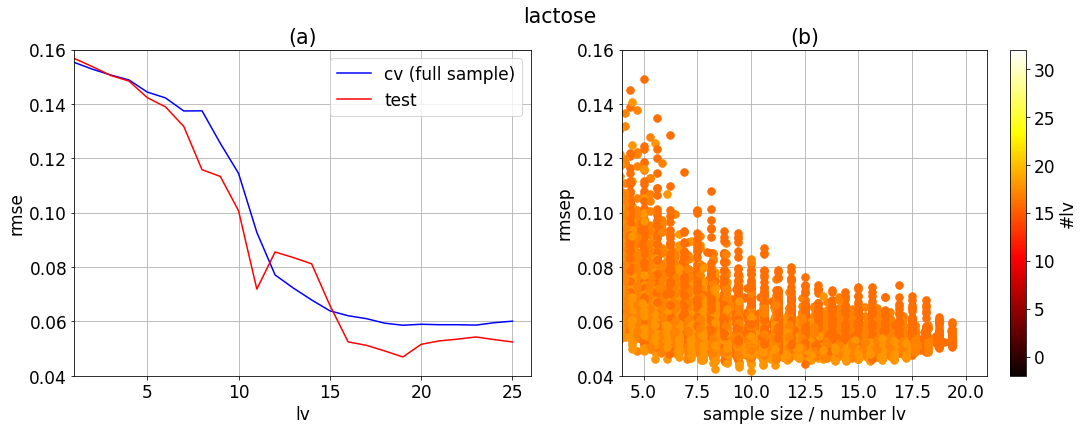
\includegraphics[width=0.42\textwidth]{manuscript/figures/d01_milk_general_framework.png}
\centering
\caption{}
\label{fig_d01_milk_general_framework}
\end{figure}

\begin{figure}[b]
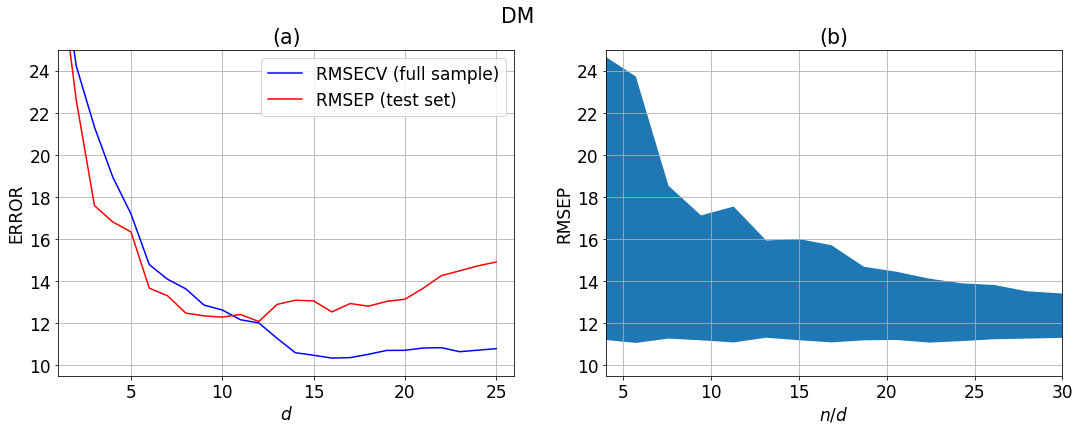
\includegraphics[width=0.42\textwidth]{manuscript/figures/d02_manure_general_framework.png}
\centering
\caption{}
\label{fig_d02_manure_general_framework}
\end{figure}

\subsection*{Specific framework}\label{results:specframework}

\begin{figure*}[t]
    \centering
    \subfigure[Milk]{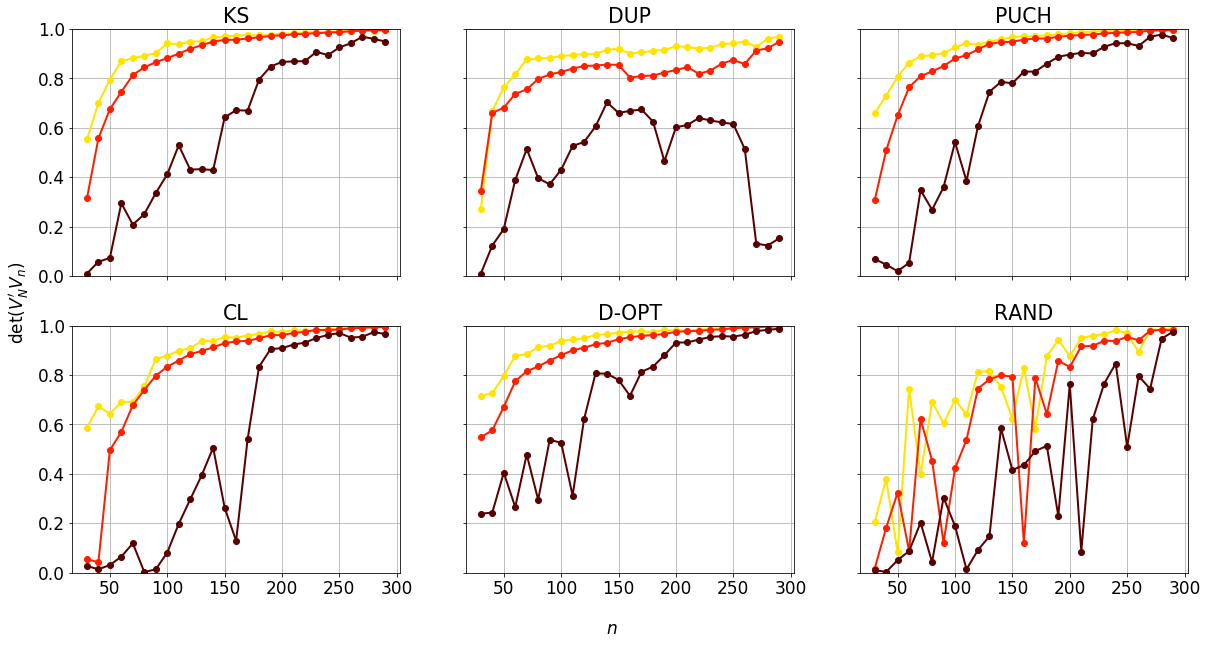
\includegraphics[width=0.4\textwidth]{manuscript/figures/d01_milk_specific_framework_detereigevect.png}} 
    \subfigure[Manure]{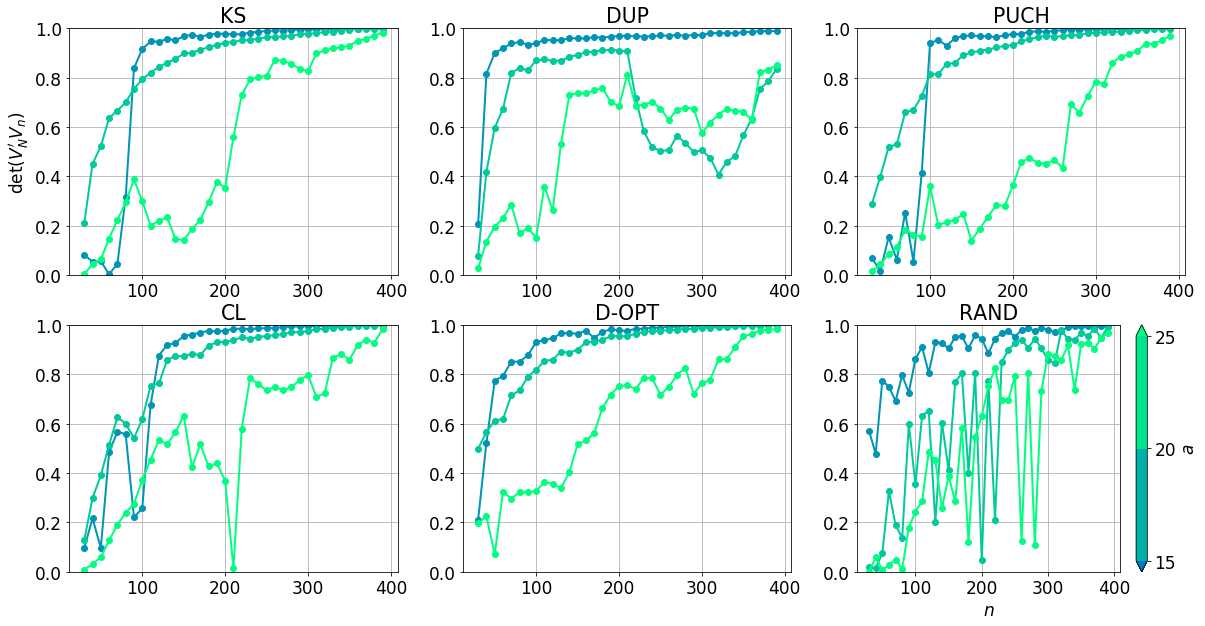
\includegraphics[width=0.4\textwidth]{manuscript/figures/d02_manure_specific_framework_detereigevect.png}}
    \caption{}
    \label{fig_specific_framework_detereigevect}
\end{figure*}

\begin{figure}[b]
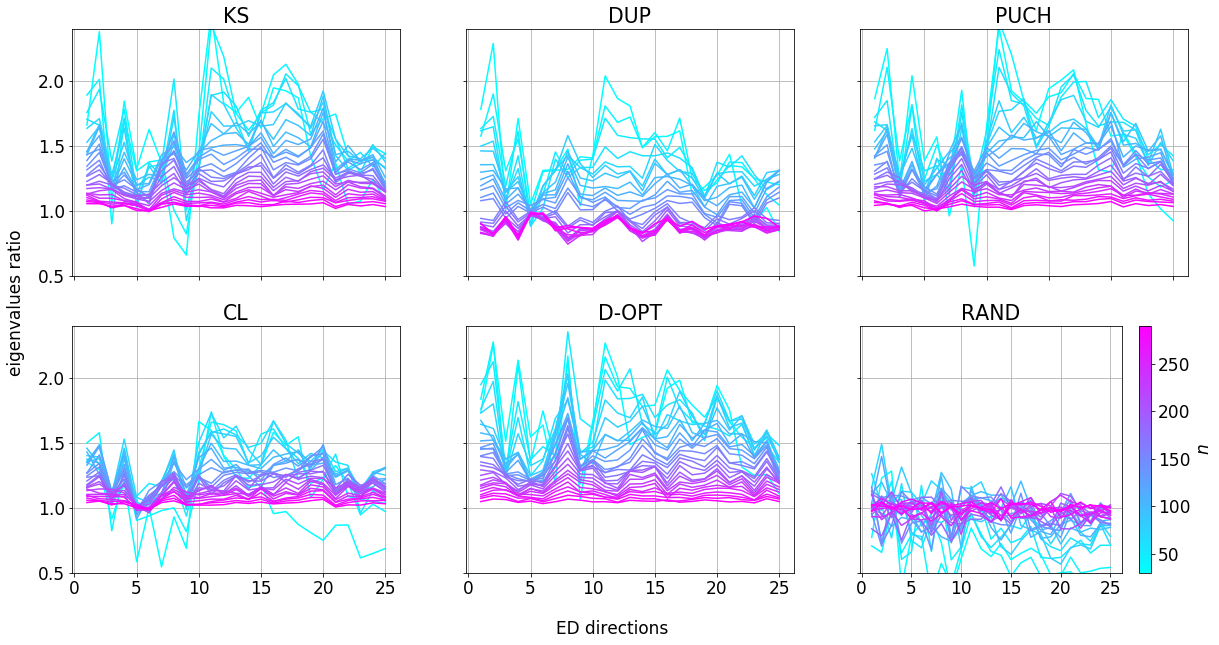
\includegraphics[width=0.42\textwidth]{manuscript/figures/d01_milk_specific_framework_eigenvalsratio.png}
\centering
\caption{}
\label{fig_d01_milk_specific_framework_eigenvalsratio}
\end{figure}

\begin{figure}[b]
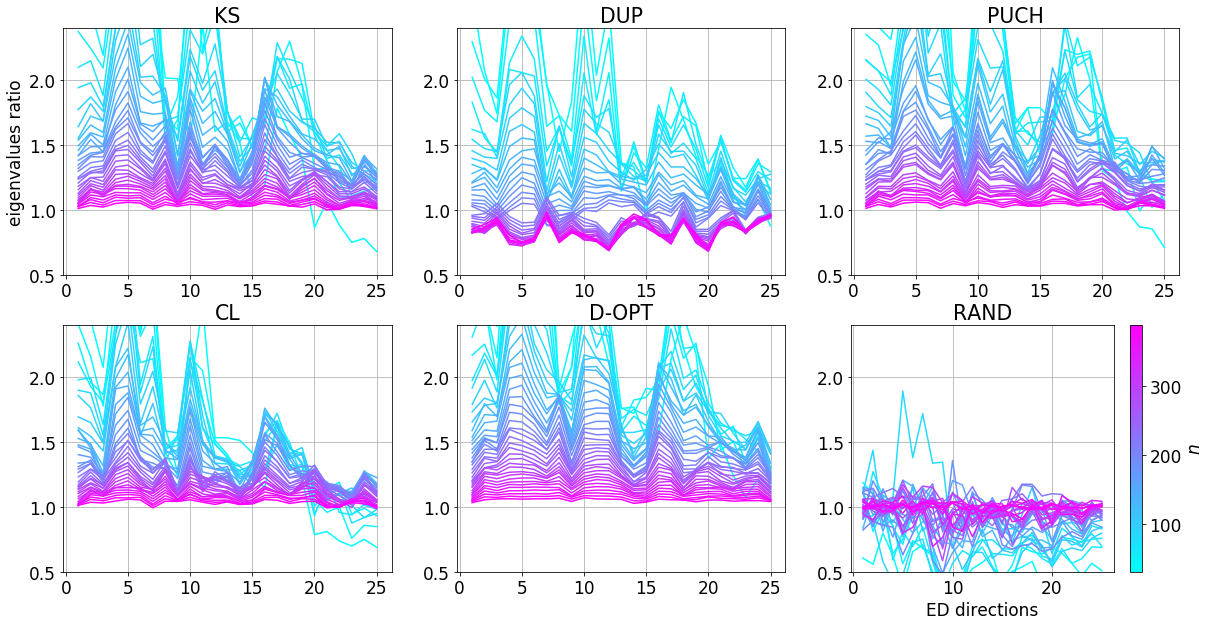
\includegraphics[width=0.42\textwidth]{manuscript/figures/d02_manure_specific_framework_eigenvalsratio.png}
\centering
\caption{}
\label{fig_d02_manure_specific_framework_eigenvalsratio}
\end{figure}

\subsection*{Model performance}\label{results:modperformance}


\begin{figure}[b]
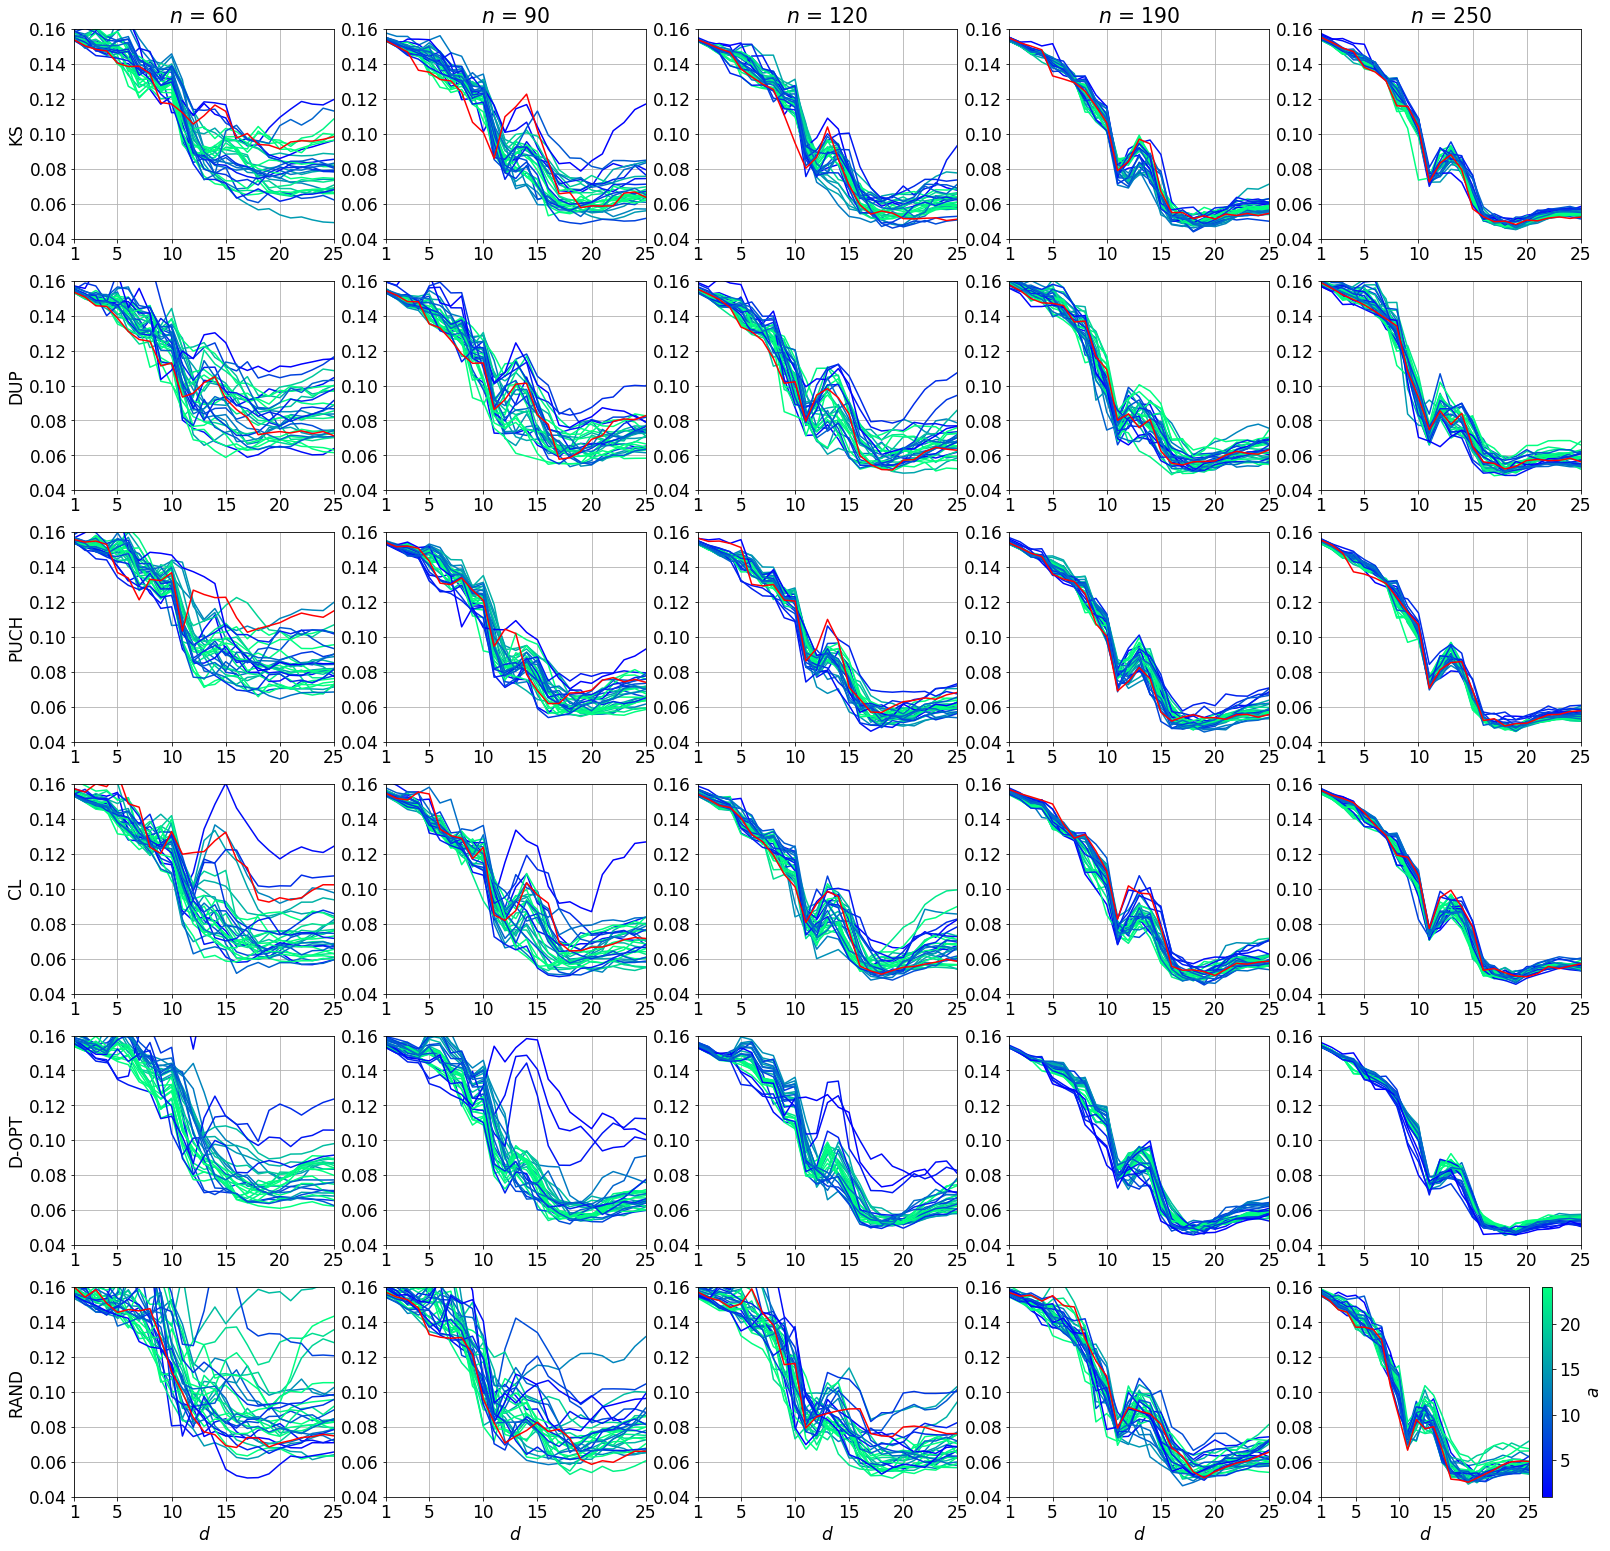
\includegraphics[width=0.8\textwidth]{manuscript/figures/d01_milk_model_performance.png}
\centering
\caption{}
\label{fig_d01_milk_model_performance}
\end{figure}


\begin{figure}[b]
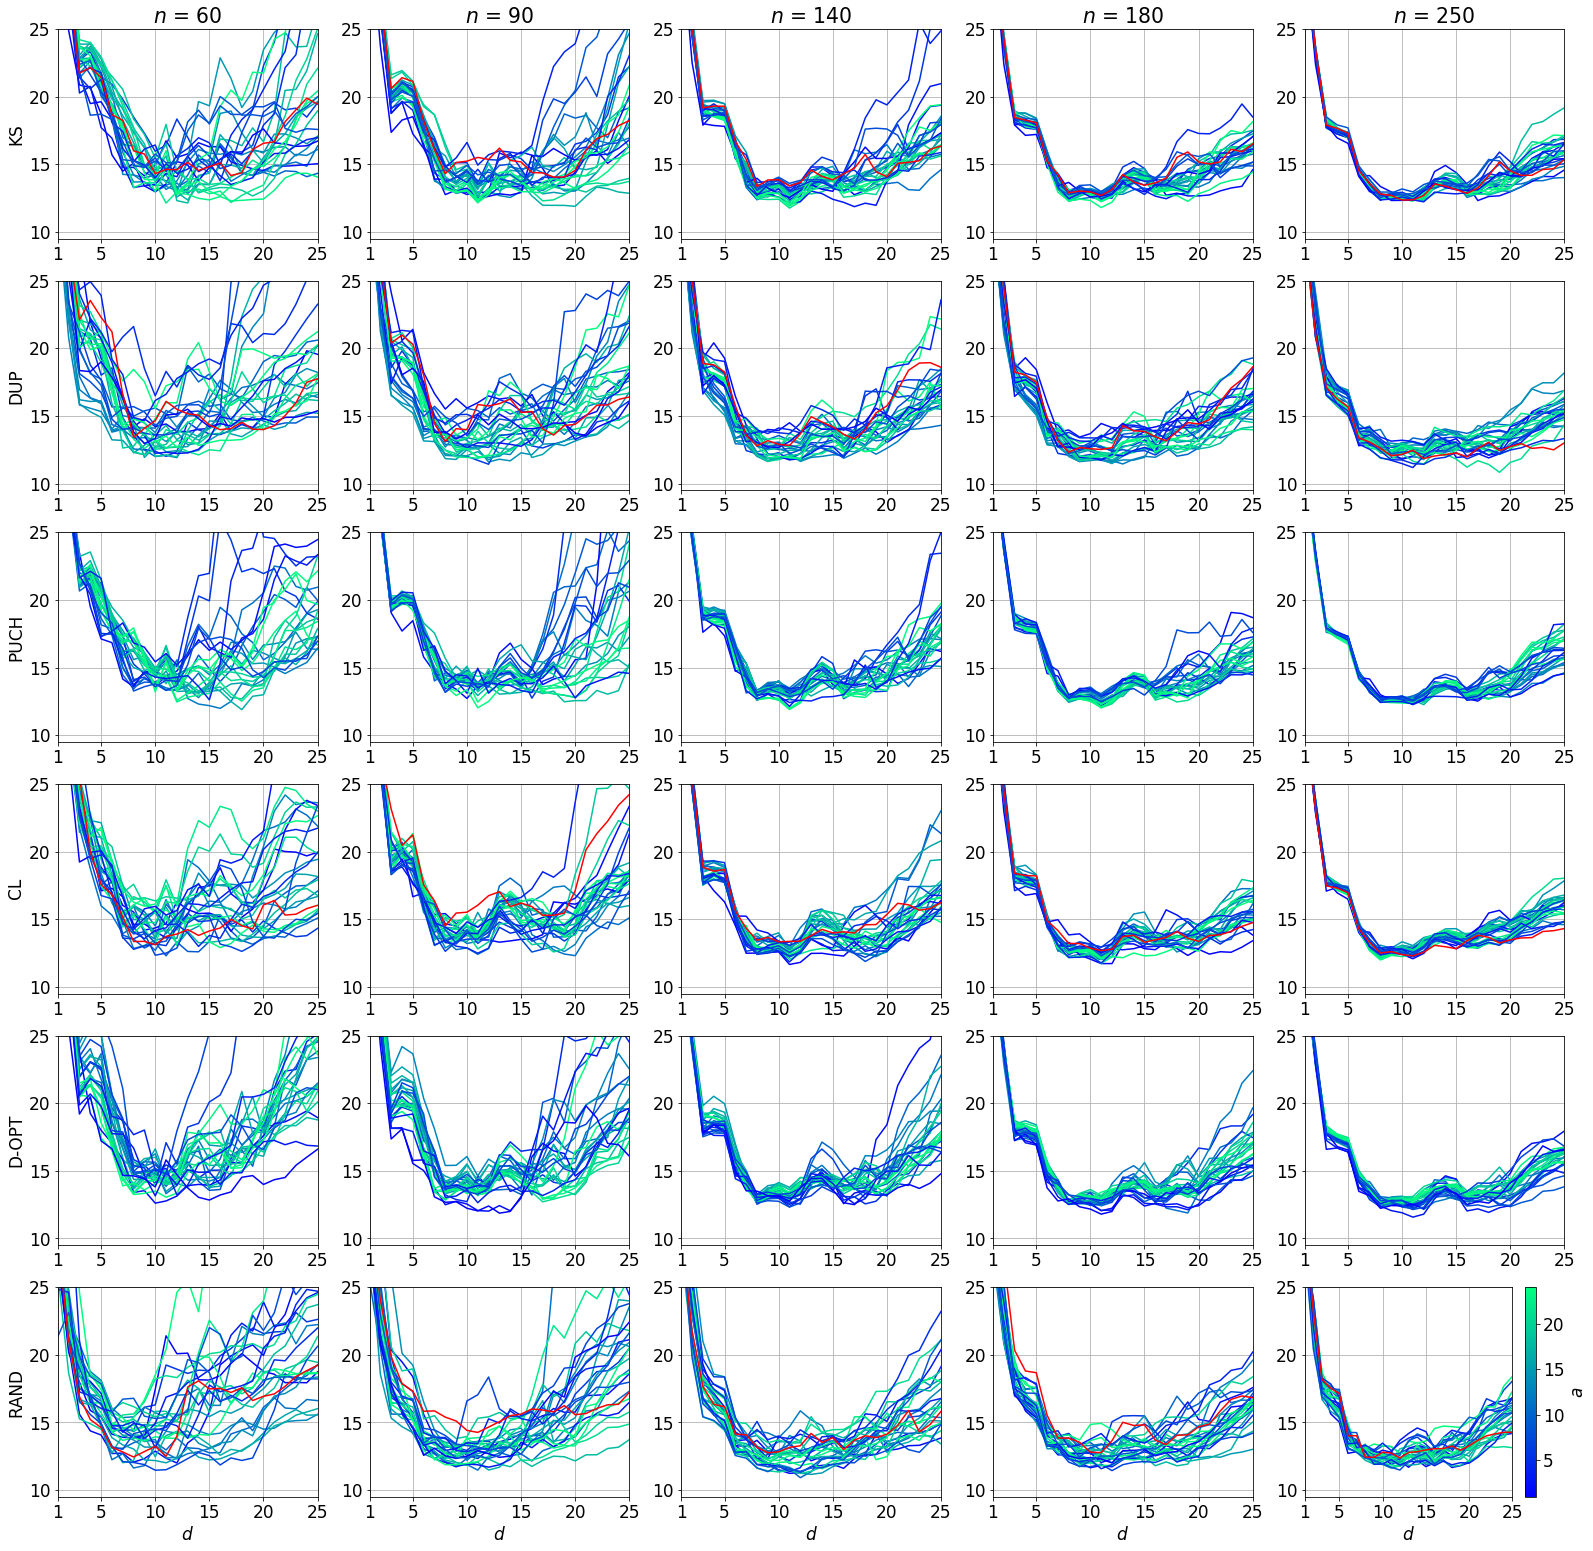
\includegraphics[width=0.8\textwidth]{manuscript/figures/d02_manure_model_performance.png}
\centering
\caption{}
\label{fig_d02_manure_model_performance}
\end{figure}


\section*{Discussion}\label{discussion}

\section*{Conclusions}\label{conclusions}

\section*{Bibliography}

\end{document}

